% Inspiré de la section 10 du papier formose

\noteFabien{metamodel ou meta-model ? perso je penche plus pour le premier}
\noteJC{pareil, j'utilise plutôt metamodel, en général}

To meet the \mpc, we have decided to use the general
approach of model federation~\cite{Golra2016-federation}. \emph{Model
  federation} is a way to assemble models using some kind of
low-coupling links. It has been studied to answer the OMG' RFP
Semantic Modeling for Information Federation (SIMF)~\cite{simf}. In
contrast to approaches that compose meta-models into a single large
meta-model grouping all needed entities, model federation build links
among models and meta-models (even through levels) to make ``things''
work together. As an illustration of this feature, we developed a
free-modeling editor -- freeing oneself from the bonds of
model/meta-model conformity -- that is presented
in~\cite{models2016-freemodel}. Another very interesting feature of
this approach is the strong decoupling among tools that remain usable
after federations are made.

We decided to use this approach since it offers the possibility to
link and to navigate among levels. Before we describe the overall
architecture in next section, here are some key concepts implemented
in the Openflexo~\cite{openflexo_link} framework.

% figure
% Dans la suite les références à la figure sont commentés

\begin{figure}
    \centering
    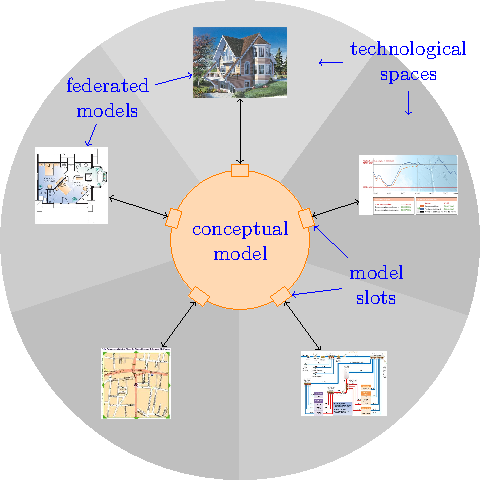
\includegraphics{Figures/federation.pdf}
    \caption{Caption}
    \label{fig:my_label}
\end{figure}

This framework relies on the following architecture. A federation
gathers a set of conceptual models, named \emph{virtual models} and a
set of \emph{federated models}. Each federated model pertains to a
\emph{technological space} and uses the language of its specific
paradigm while a virtual model is built using the Flexo Modeling
Language (FML). Each federated model can be viewed as an autonomous
component that may evolve with its own tooling. The virtual models
serve as control components.


FML is a language designed to define virtual models. A virtual model
is composed of a set of \emph{concepts}, while itself being a concept.
Hence, virtual models are structuring units while concepts are the
core entities. A concept has a set of \emph{roles} and
\emph{behaviors}. A parallel to object-oriented approach can be useful
to understand FML\footnote{Beware, even though useful for
  comprehension, this correspondence is not
  reliable, as some aspects of FML do not map to object oriented
  concepts}. A concept corresponds to a class, its roles to the
attributes of the class and its behaviors to the methods of the class.
These roles have types defining the kind of value the role will point
at runtime.
Whenever a type external to the federation space (from a TA or an
external model) is used, one needs to use a \emph{model slot}. A model
slot is a mediation entity, associated with a TA, in charge of giving
access to external elements of the corresponding technological space.

A \emph{technology adapter} (TA) is a reusable library that defines
connections between the FML execution engine and a particular
technological space. The model federation framework provides ways to
define TA.

We should stress that building a virtual model is purely conceptual,
model slots / TA are in charge of the technicalities. Additionally,
when a virtual model or a concept point to an external model, it comes
with an explicit interpretation of the external data. The virtual
model can hide information, transform elements and does not need to
cover the whole external metamodel.
% In our example, it ignores all other elements of the \smk metamodel.
We did not required TA in our proposal. The whole solution uses the
internal (FML) language.

FML is designed to define not only the structure of virtual models but
also to define the collection of actions an engineer can perform on
them. These actions are called \emph{business behaviors} and may be
compared to methods of object-oriented approach.
% The rename operation already cited for the \textsf{Goal-xls}
% federation is an example of such a behavior. One could also define
% operations to add or remove requirements, to refine relationships,
% \emph{etc.} The renaming operation is defined by a \texttt{rename}
% behavior in the concept \texttt{Requirement}. It uses the
% \texttt{setCell} action of the Excel TA and the \texttt{rnGoal} of
% the \smk TA.
When the FML execution engine runs a federation, it creates virtual
model instances containing concept instances. Some concept instances
are connected to external elements through model slot instances.
% The lower part of the figure~\ref{fig:space-ex} illustrates this
% runtime phase.

FML also supports another kind of behavior which can be described as
interactors. Such behavior is reactive and triggers when any of the
federated models evolves. Two scenarios are then possible: (1) an
action in the federation is propagated to the federated models or (2)
a modification is detected in a federated model and triggers a
behavioral interactor of the federation.
% Hence the double arrows in the links of Figure~\ref{fig:space-ex}.
This feature is useful when models have to be synchronised. We did not
exploit this possibility in the challenge.

The tool support for model federation framework,
Openflexo\footnote{\url{https://github.com/openflexo-team}}, is
developed as an open source initiative. This tool offers a FML
execution engine with an interactive virtual model design environment.
It has been used in several case studies including model mapping,
multi-paradigm process modeling and enterprise architecting. It has
also been used to build a tool, the freemodeling editor that has been
used in industrial projects~\cite{models2016-freemodel}. As of today, this tool
offers some mature technology adapters (\emph{docx} and \emph{excel}
for documents, EMF and OWL for modeling languages, JDBC for databases,
REST and XMLRPC for external services and one for diagramming tools)
and other more rudimentary (pdf, HTTP, XML, etc.).

Finally, tools have their own model. We have taken advantage of
Openflexo features to build, in parallel with the models and virtual
models required by the challenge, a drawing tool that makes our
solution (partially) executable.
